\section{Results}
\label{results}

\subsection{Learned Material Parameters}

\begin{figure}[t]
    \centering
    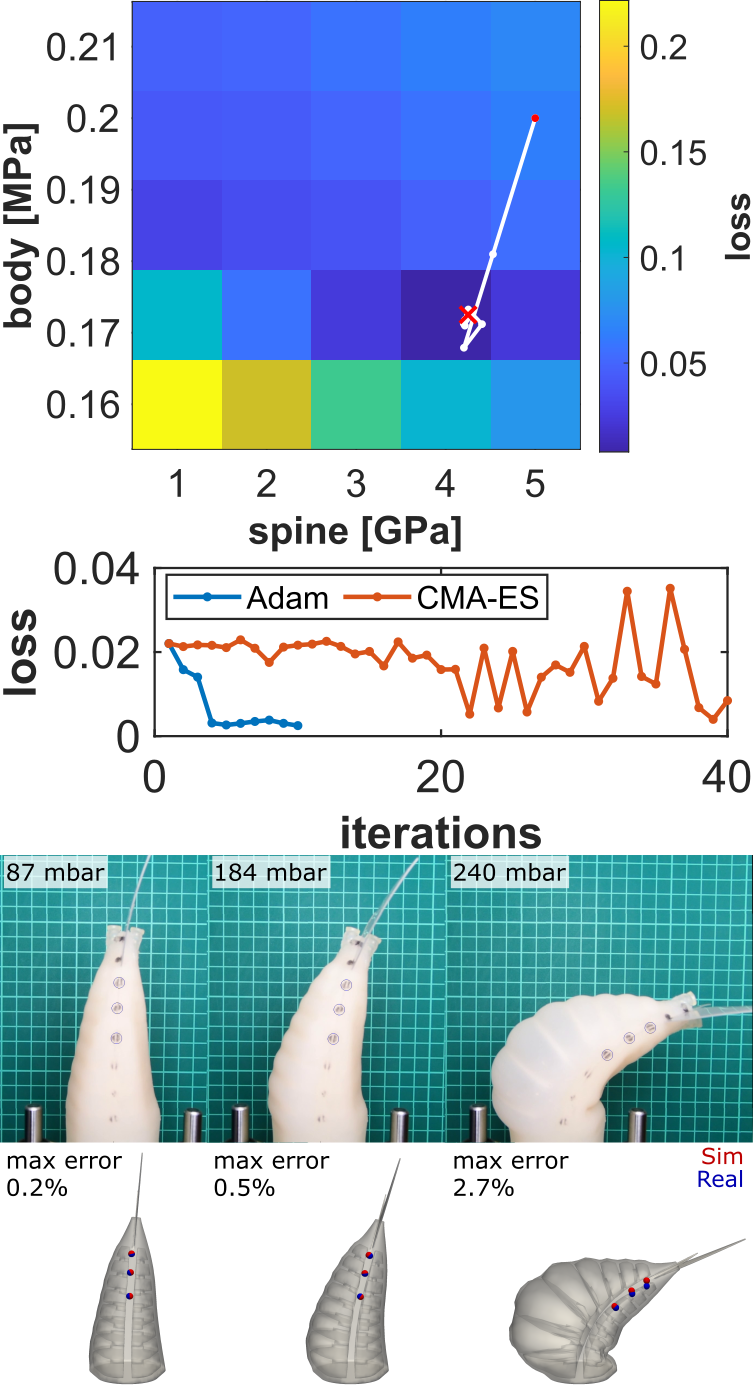
\includegraphics[width=0.85\columnwidth]{figures/grid_search_nemo_vertical_column.png}
    \caption{\textit{Top:} Exhaustive search of the Young's moduli pair for the spine and body. The moduli pair with the lowest Euclidean loss is located at the red $\times$. The red dot indicates the start of a gradient search and the white line shows the progress towards convergence. \textit{Middle:} Convergence comparison between a gradient-based (Adam) and gradient-free search (CMA-ES). \textit{Bottom:} Comparison of static deformation of the \emph{Nemo} fish for increasing pressure in experiment and simulation. Maximum displacement error increases with pressure, but remains within the measurement error (on the order of the diameter of markers). The grid in white under the real robot has \SI{10}{mm} spacing. The reported error is normalized to the fish tail length of \SI{10}{cm}.}
    \label{fig:system_id}
\end{figure}

\begin{figure}[t]
    \centering
    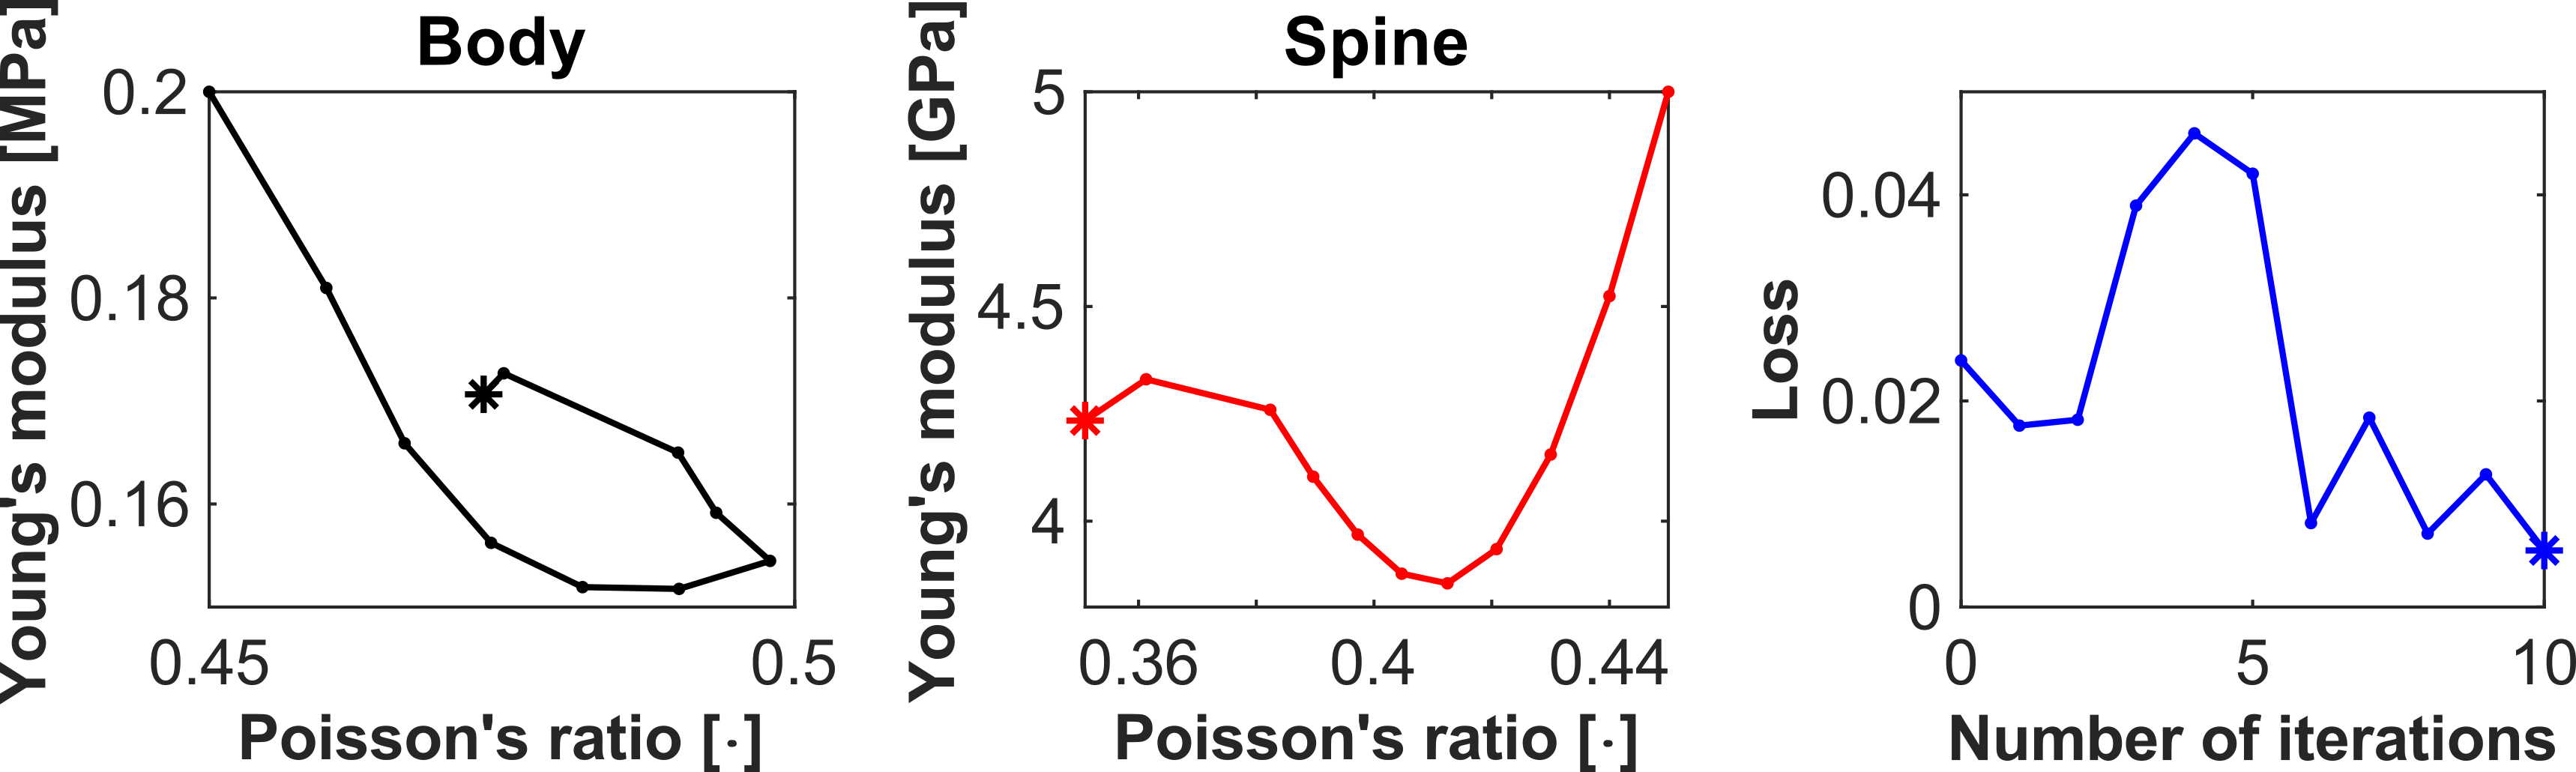
\includegraphics[width=0.99\columnwidth]{figures/param_search_figure_new.png}
    \caption{Learning four material parameters from deformation data take with the \textit{Nemo} fish prototype using a gradient-based approach that is run until convergence. The final values for Young's moduli and Poisson's ratios depicted as an asterisk agree with plausible material parameter values with lower loss.}
    \label{fig:4_param_search}
\end{figure}

For the \emph{Nemo} tail actuator described in \Cref{tab:fish}, we perform a grid search of the loss landscape centered around the ground truth datasheet values for the silicone and acetal materials of the body and spine. We report that if the exact geometry of the actuator is reproduced with high fidelity in the simulation, we converge to values within the range of typical measured values for the material Young's moduli (see \Cref{fig:system_id}). Further, we see that there is a unique minimum value that is within the acceptable range of measured moduli for both parameters. Note that we assume a priori that the Poisson ratio for silicone is $\nu\approx0.5$ or \textit{nearly} incompressible, a standard assumption for silicone, and the acetal sheet Poisson ratio is $\nu=0.37$ as reported by the manufacturer. Typical values for the Young's modulus of Dragon Skin 10 range from \SI{0.1}{MPa} to \SI{0.25}{MPa} and the value for Dragon Skin 20 was measured to be in the range of \SI{1.1}{MPa}~\cite{marechal2020toward} and typical values for the Young's modulus of acetal sheets range from \SI{2.5}{GPa} to \SI{5}{GPa}.\footnote{\url{https://dielectricmfg.com/knowledge-base/acetal/}}

In \Cref{fig:4_param_search}, we demonstrate that our method can be extended to higher dimensional parameter spaces such as a search over both Young's moduli and Poisson's ratios. Note that although we allow the Poisson ratio to vary in this identification experiment, the final value to which the body Poisson's ratio converges is still \textit{nearly} incompressible as expected for silicone.


\subsection{Gradient-based and Gradient-free Solver Methods}

We compare the runtime of the gradient-free method \emph{CMA-ES} against the runtime of the gradient-based method \emph{Adam} in \Cref{tab:gradient_methods}. The comparison shows that although \emph{CMA-ES}~\cite{igel2007covariance} is slightly faster in runtime per iteration, the use of the gradient-based method Adam~\cite{kingma2014adam} is significantly more effective for convergence. These comparative experiments shown in \Cref{fig:system_id} were carried out on a computer with an Intel Core i9-9900K @ 3.60GHz with 16 cores processor and 64.0 GB of memory.

\begin{table}[htb]
    \centering
    \caption{Comparison of Adam, CMA-ES, and Grid search. The forward simulation time is 318.9 seconds equivalent to grid search.}
    % \begin{tabular}{|p{10mm}|p{12mm}|p{12mm}|p{10mm}|p{17mm}|}
    \begin{tabular}{@{}lllll@{}}
        \toprule
        \thead[l]{Method} & \thead[l]{Total\\Iterations} & \thead[l]{Time Per\\ Iteration} & \thead[l]{Total Time} & \thead[l]{Loss After \\4 Iterations} \\
        \midrule
        \textbf{Adam} & \textbf{4} & 334.4 s & \textbf{~22 m} & \textbf{0.0027} \\
        CMA-ES & 40 & 321.0 s & ~214 m & 0.021  \\
        Grid search & 25 & \textbf{318.9 s} & 132.9 m & 0.023 \\
        \bottomrule
    \end{tabular}
    \label{tab:gradient_methods}
\end{table}

\subsection{Dynamic Experiments}

For dynamic experiments, we compare the results of our simulation output with the measured data of the furthest tracked dot on the tail. In Fig.~\ref{fig:results}, we report our findings for sim2real performance in both the standard fish (\emph{Nemo}) and two other data sets for a tail with different Young's moduli for the body (\emph{Bruce}) and a tail with a greater number of air chambers (\emph{Dory}). We demonstrate that if system identification is done correctly our simulation results can predict the performance of a novel actuator design to within millimeter precision or $3\%$ max normalized error using only a quasistatic data set for training without need for material testing. The \textit{Bruce} prototype required higher pressures to get similar displacements to \textit{Nemo} since the material is stiffer. The prototype \textit{Dory} required higher pressure as well to produce similar displacements due to a greater number of actuation chambers. For videos of the dynamic experiments and simulation, we ask readers to refer to our supplemental video.

\begin{figure}[t]
    \centering
    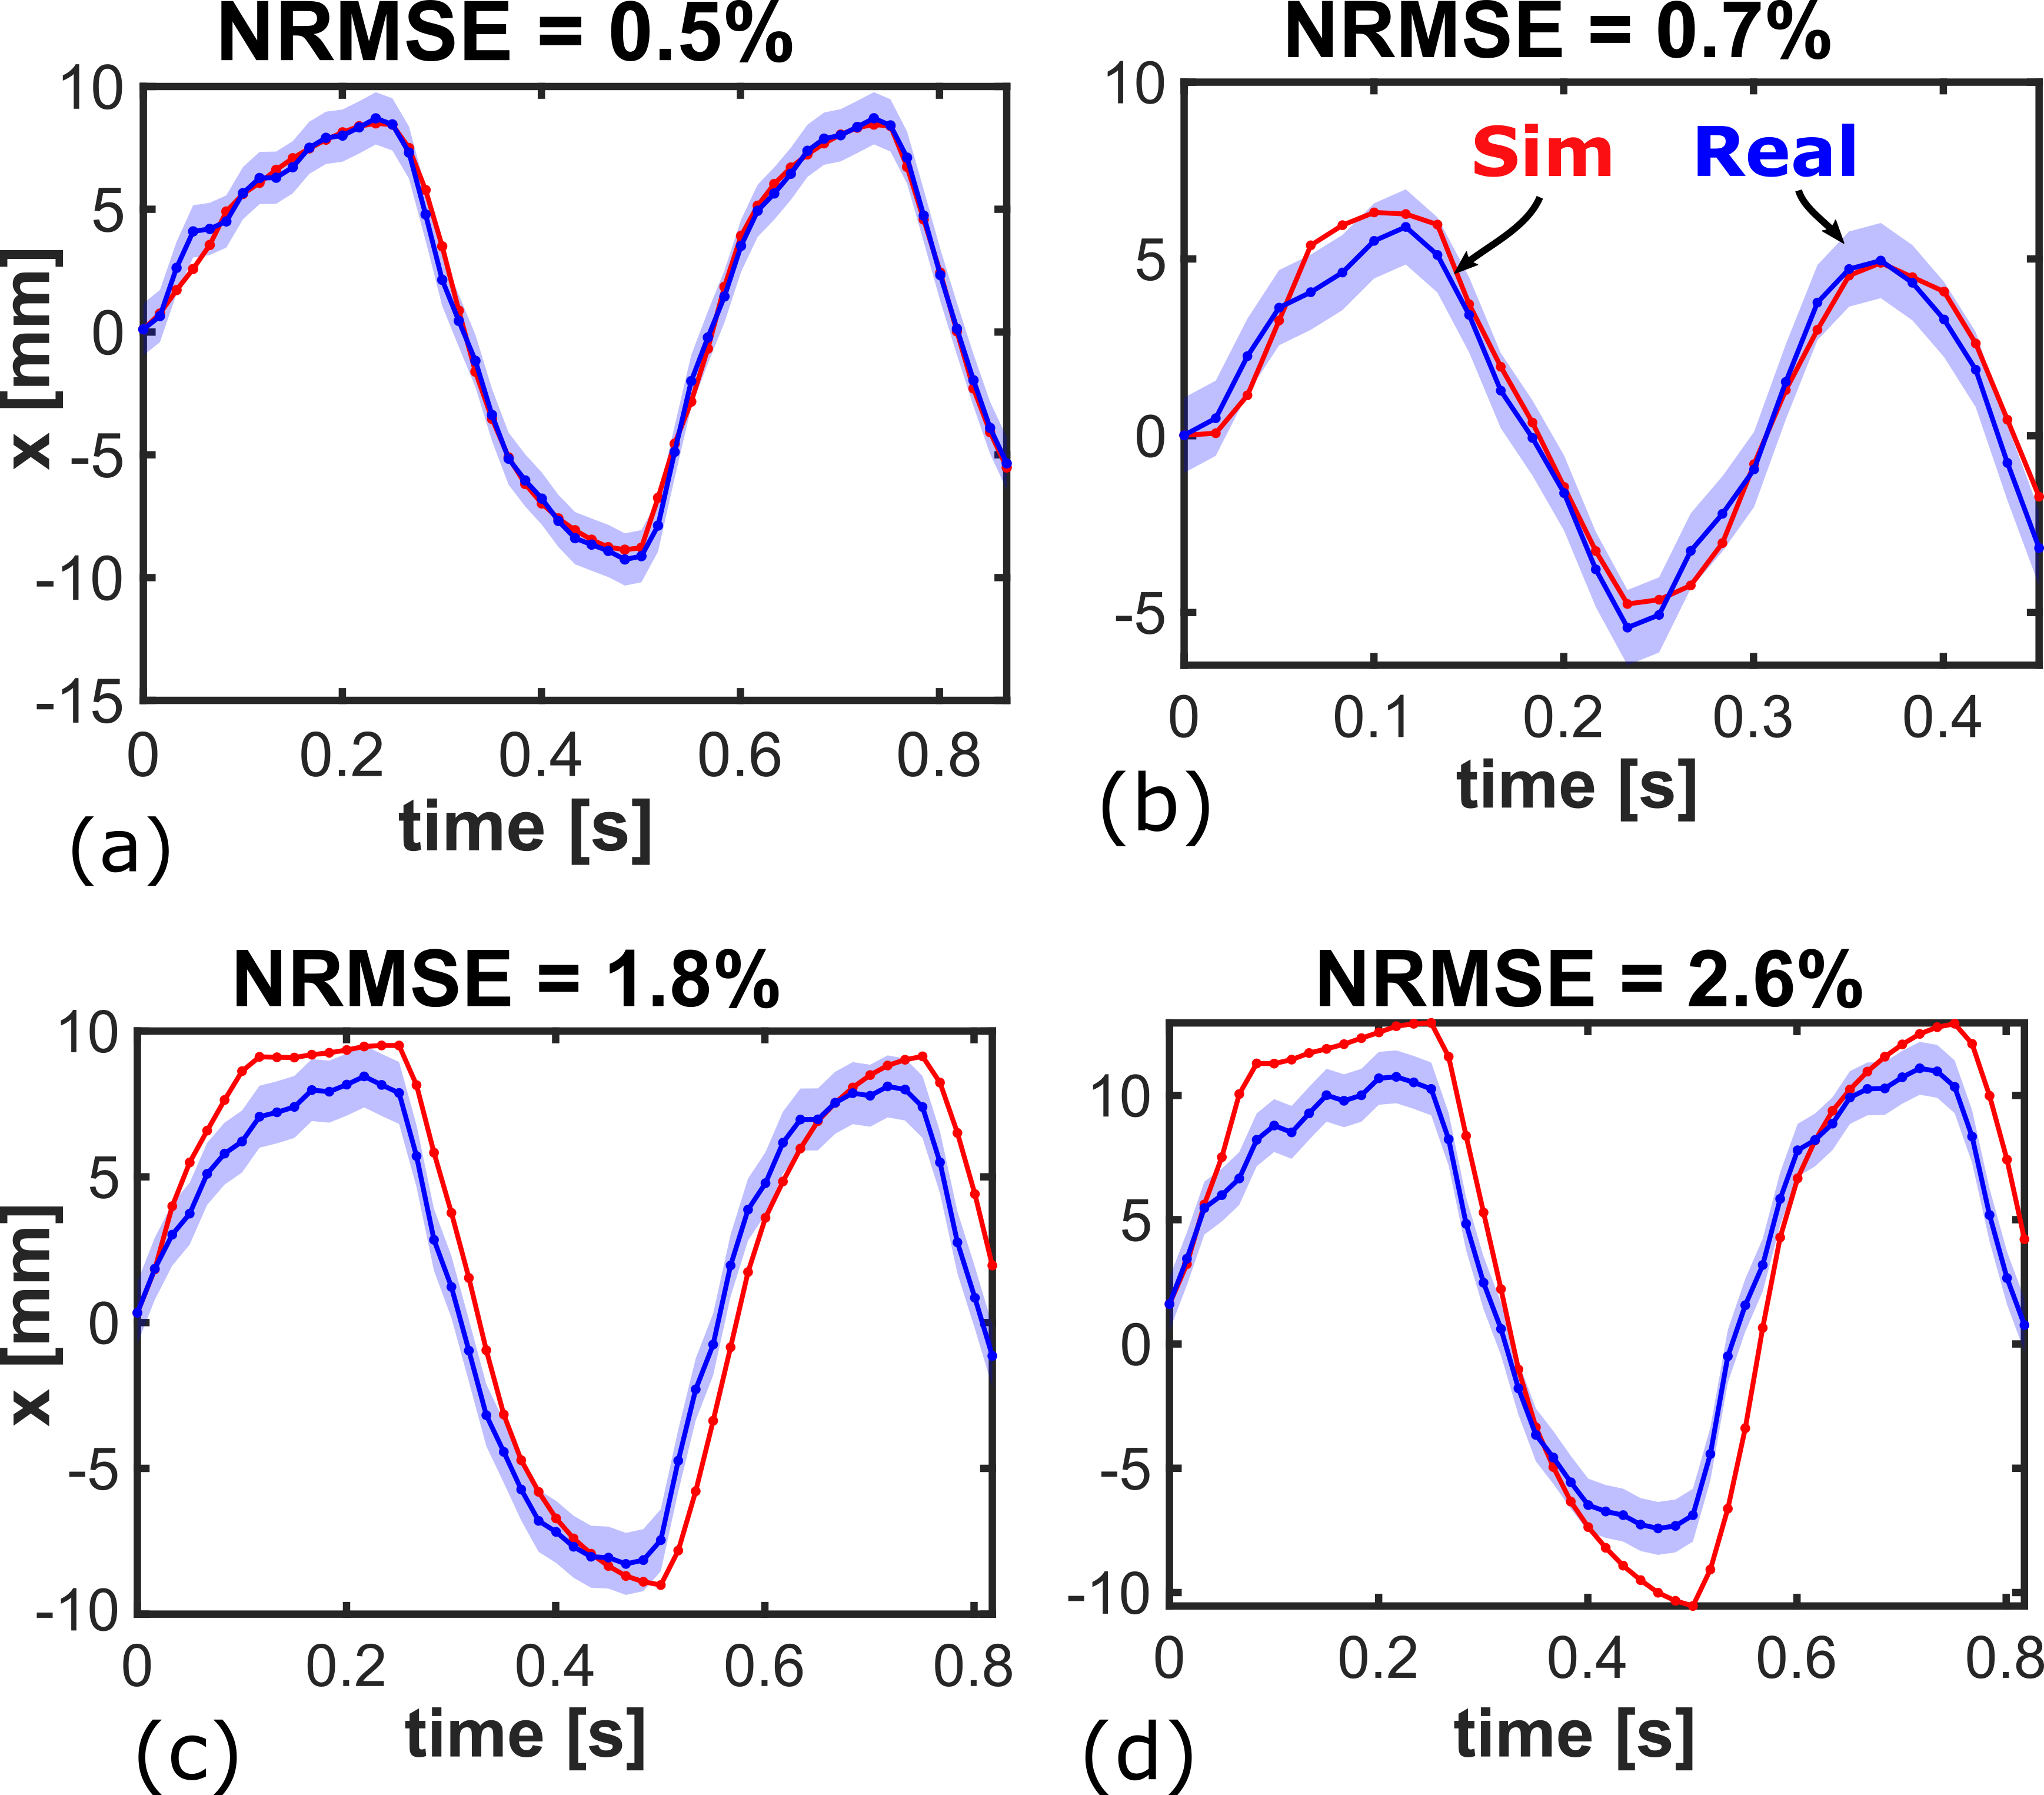
\includegraphics[width=0.85\columnwidth]{figures/dynamic_actuation_square.png}
    \caption{Simulation and measurement data for the \emph{Nemo} fish at (a) 200 mbar and 2 Hz, (b) 200 mbar and 4 Hz, (c) the \emph{Bruce} fish at 500 mbar and 2 Hz, and (d) the \emph{Dory} fish at 350 mbar and 2 Hz. The color bands indicate the variance from $N=5$ trials. For both actuation signals, we are capable of achieving sub-millimeter accuracy between experiment and simulation. The same method is used to identify the parameters of Bruce and Dory, exhibiting accuracy still within \SI{3}{mm}. We normalize the Root Mean Square Error (RMSE) to the fish tail length of \SI{10}{cm}. As expected, higher pressures result in larger deformations with greater error. The phase lag exhibited in \emph{Bruce} and \emph{Dory} may be due to actuator dynamics present during higher actuation pressures.}
    \label{fig:results}
    \vspace{-3pt}
\end{figure}

\subsection{Learned Hydrodynamics}
\label{sec:learned_hydrodynamics}
We compare our simple predictor of thrust force with the measurement data and the theoretical thrust from EBT, a classic, non-learning-based approximate analytical model from the literature, in~\Cref{fig:thrust_prediction}. Although the model is capable of generalizing to actuation signals at frequencies previously unobserved in the training for the \emph{Nemo} prototype, for the \emph{Bruce} prototype the discrepancy is large, nearly twice the measured force, likely because of the more limited training data.
In comparing to the thrust prediction from EBT, we see that the analytical thrust is strictly positive. The negative measured force is due to recoil of the measurement system. The advantage of our approach is the differentiability and flexibility of the neural network provided enough data is collected. We note that the network is capable of learning the measurement dynamics due to the compliance of the load cell and the damping of the water though these effects can be considered separately and corrected for if desired (see \Cref{sec:load_cell_measurement}). We conjecture that the asymmetry of the measured thrust may be due to imperfections in the fabrication process of the fish tails favoring one direction more strongly.

\begin{figure}[t]
    \centering
    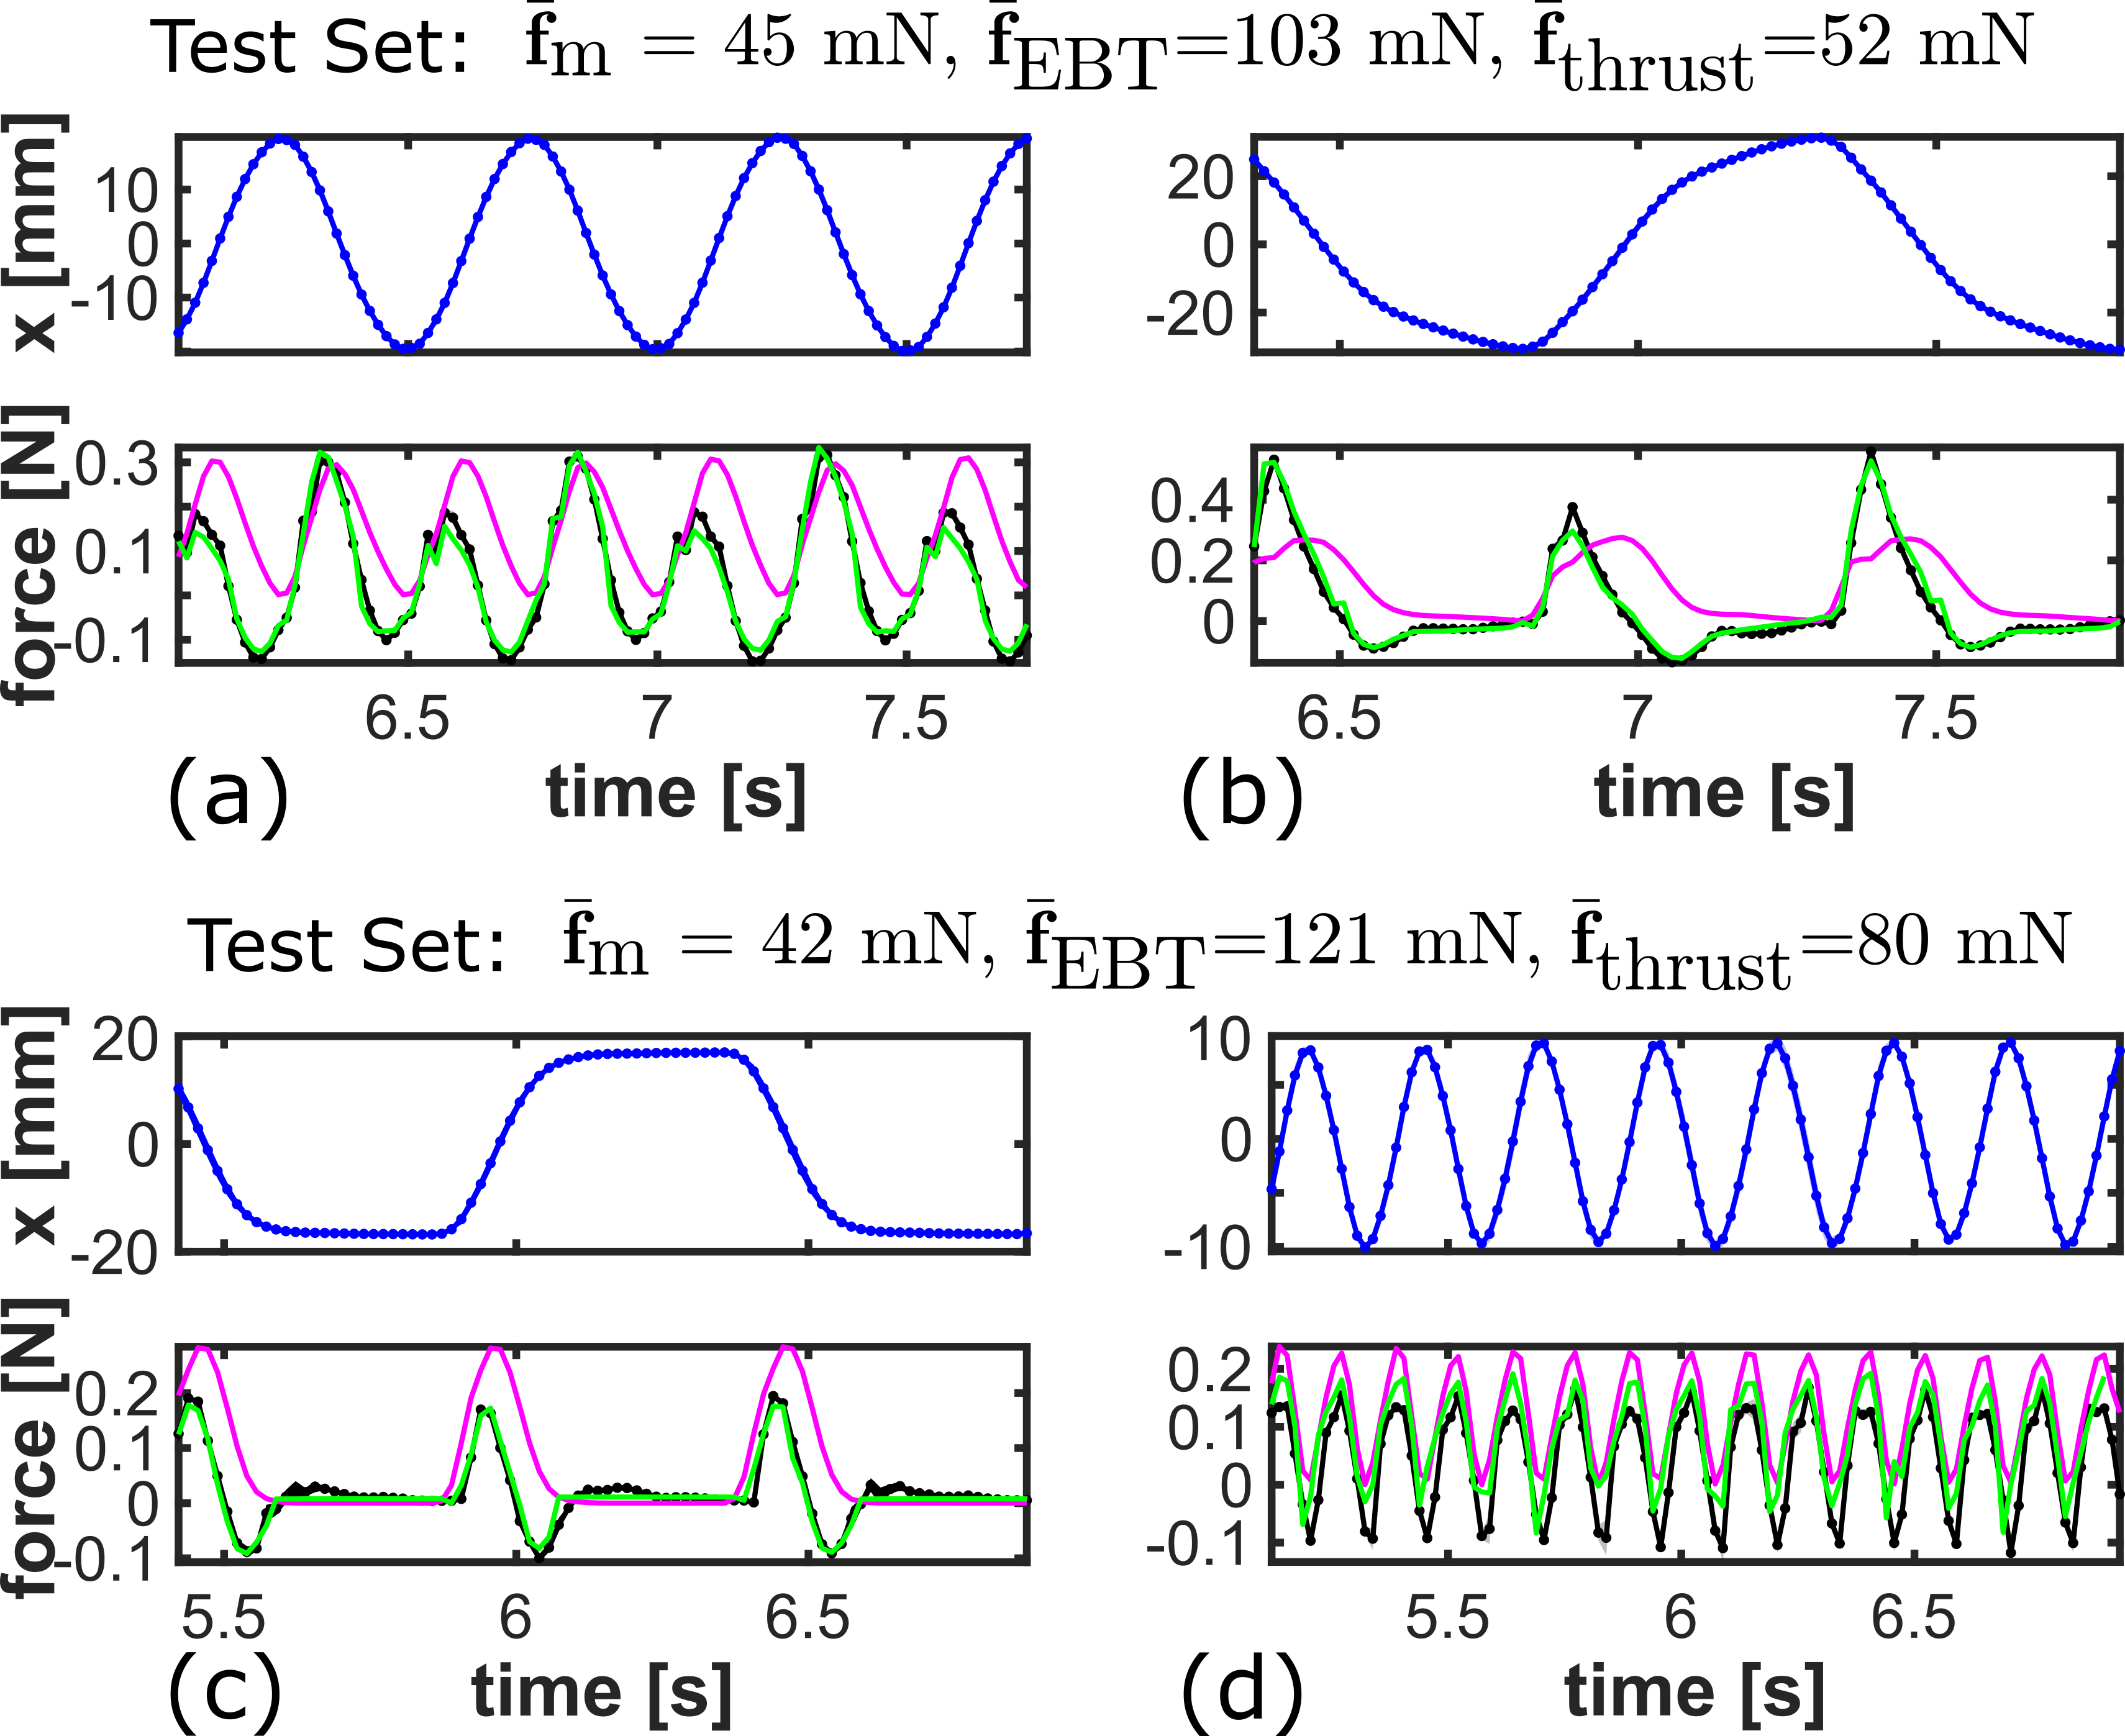
\includegraphics[width=1\columnwidth]{figures/hydrodynamics.png}
    \caption{Tail lateral displacement (blue) with thrust measurement and prediction. We compare the measured thrust force $\mathbf{f}_\textrm{m}$ (black), analytical thrust force from EBT $\mathbf{f}_\textrm{EBT}$ (magenta), and the neural network thrust prediction $\mathbf{f}_\textrm{thrust}$ (green). We show the thrust prediction for two training sets (a) and (c) and we report the time-averaged thrust for the two test cases (b) and (d). We note that EBT tends to over-predict the thrust measurement while our neural network thrust prediction accurately reproduces the frequency for a given actuation signal and matches amplitude more robustly than EBT.}
    \label{fig:thrust_prediction}
\end{figure}
